\chapter[Supporting Information for ``Tonian paleomagnetism from South China permits an inclusive Rodinia or Bitter Springs Stage true polar wander, but not both''][Supporting Information - Xiajiang Group]{Supporting Information for ``Tonian paleomagnetism from South China permits an inclusive Rodinia or Bitter Springs Stage true polar wander, but not both''}

\begin{figure}[h!]
    \centering
    \includegraphics[width=0.8\textwidth]{figures/Xiajiang/bootstrap-CDF.pdf}
    \caption[Results of the bootstrap fold test for the Xiajiang Group high-temperature component.]{Results of the bootstrap fold test \citep{Tauxe1994a} for the Xiajiang Group high-temperature component. The tightest grouping of site mean directions is obtained between 68 and 103\% unfolding at the 95\% confidence level. Since this range encompasses 100\%, the high-temperature component passes the fold test, constraining the high-temperature component to have been acquired prior to Mesozoic folding of the Xiajiang Group \citep{Li2016c, Ma2019a}.}
    \label{fig:bootstrap-CDF}
\end{figure}

\begin{figure}[h!]
    \centering
    \includegraphics[width=0.9\textwidth]{figures/Xiajiang/tuff-photos.jpg}
    \caption[Photographs of tuffs in the Xiajiang Group.]{Photographs of tuffs that yielded consistent and concordant CA-ID-TIMS $^{206}$Pb/$^{238}$U zircon dates. Red arrows point to the sampled tuffs. \textbf{A)} H2-470. \textbf{B)} H3-60. \textbf{C)} H3-8. \textbf{D)} QR-74. \textbf{E)} L4-2. No photograph is available for sample L1-27.}
    \label{fig:tuff-photos}
\end{figure}

\begin{figure}[h!]
    \centering
    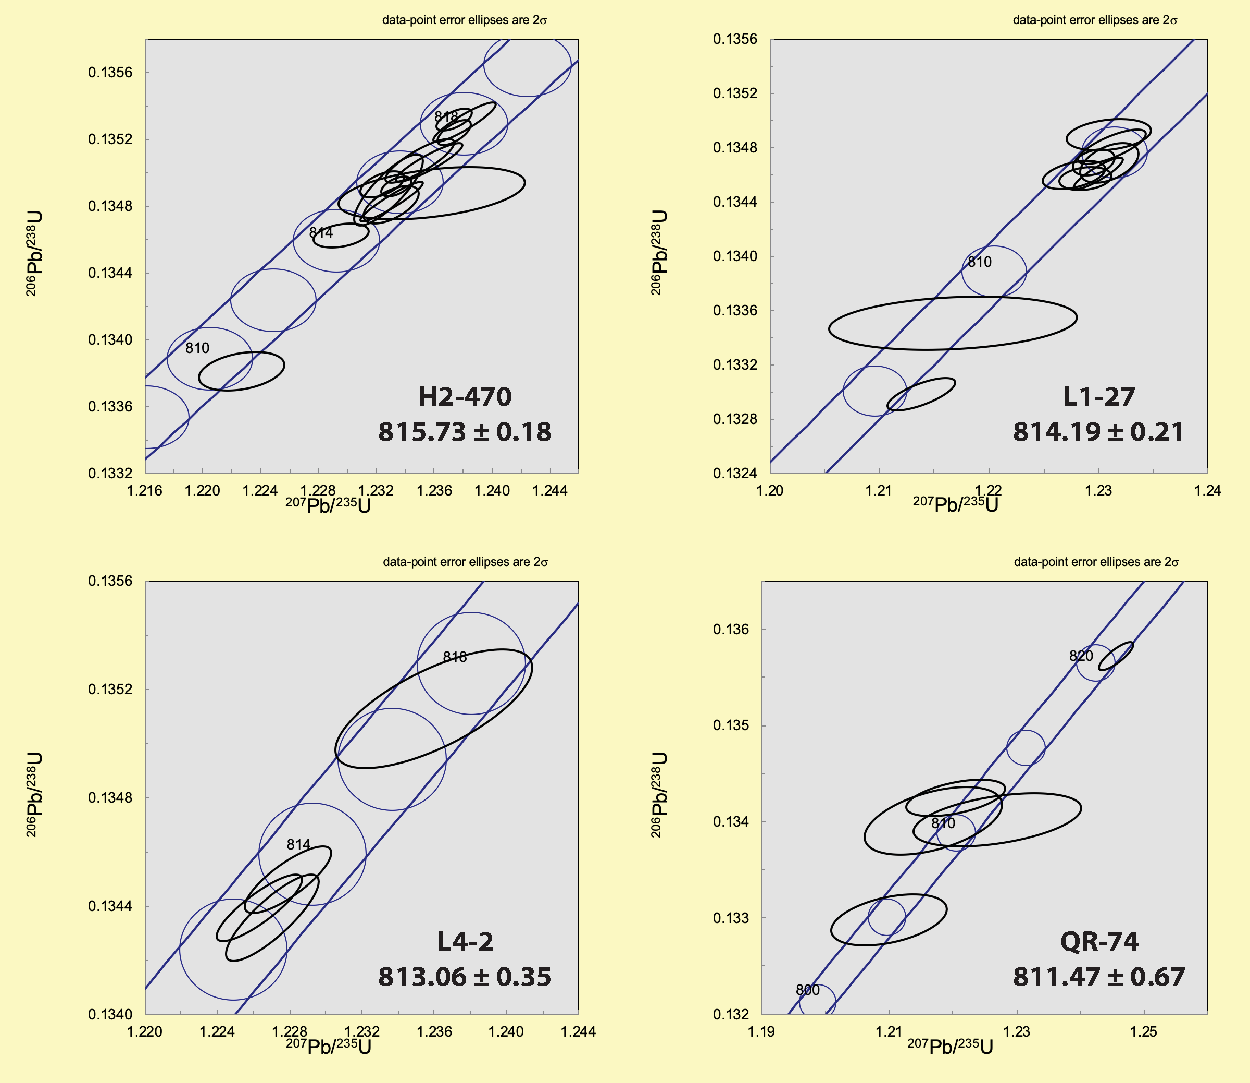
\includegraphics[width=0.9\textwidth]{figures/Xiajiang/concordia-1.pdf}
    \caption[Concordia diagrams for zircons from tuffs of the Xiajiang Group.]{Concordia diagrams for zircons from tuffs of the Xiajiang Group analyzed in this study. Individual zircon data are tabulated in Table SX.}
    \label{fig:concordia-1}
\end{figure}

\begin{figure}[h!]
    \centering
    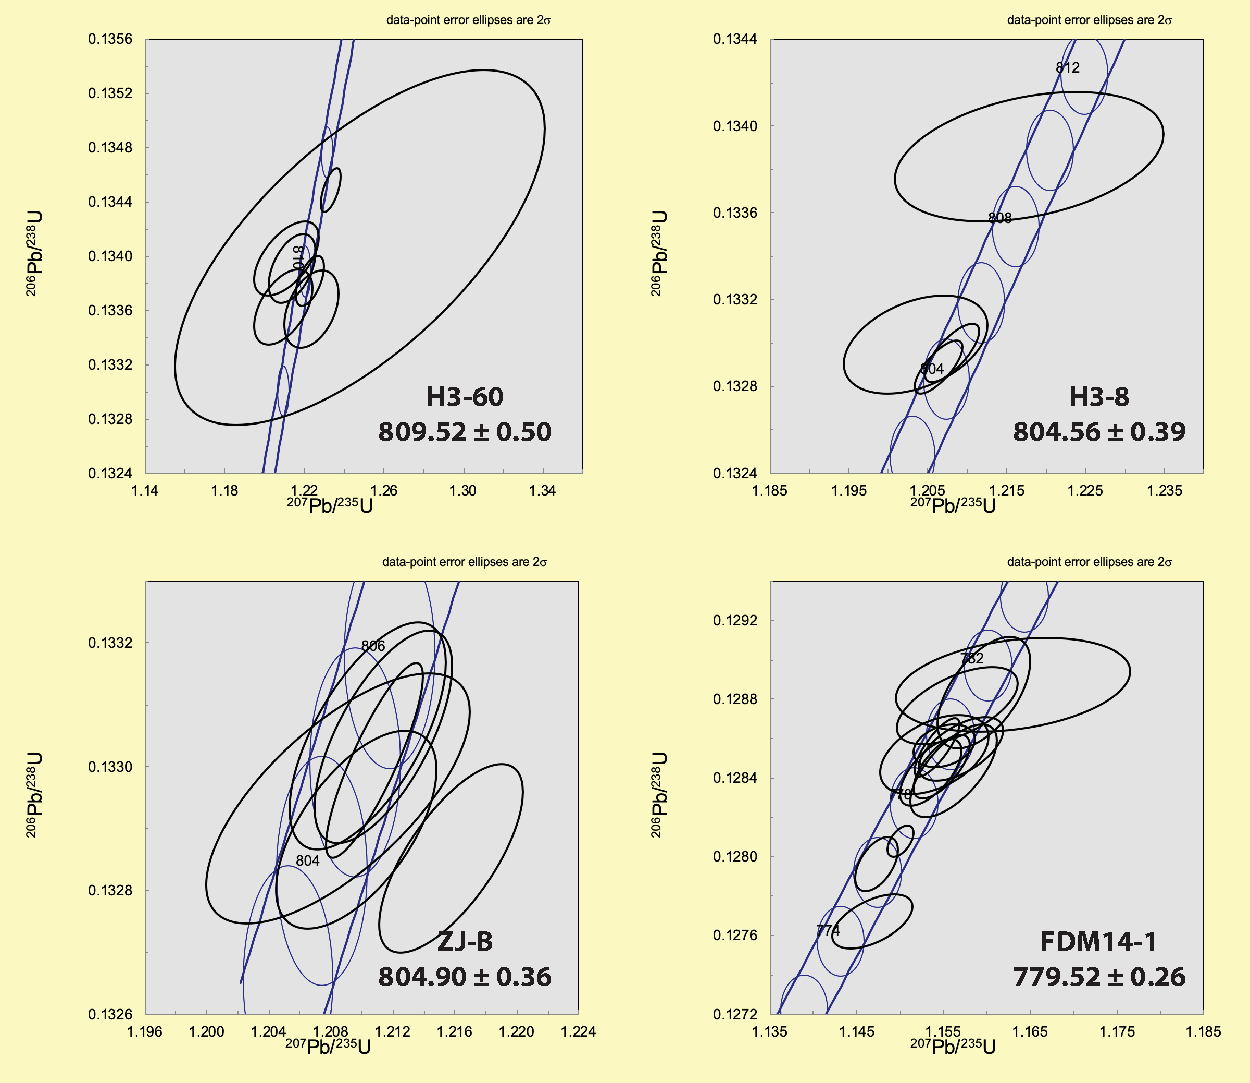
\includegraphics[width=0.9\textwidth]{figures/Xiajiang/concordia-2.pdf}
    \caption[Concordia diagrams for zircons from tuffs of the Xiajiang Group, Madiyi Formation, and Liantuo Formation.]{Concordia diagrams for zircons from tuffs of the Xiajiang Group (H3-60 and H3-8), Madiyi Formation (ZJ-B), and Liantuo Formation (FDM14-1) analyzed in this study. Individual zircon data are tabulated in Table SX.}
    \label{fig:concordia-2}
\end{figure}

\begin{figure}[h!]
    \centering
    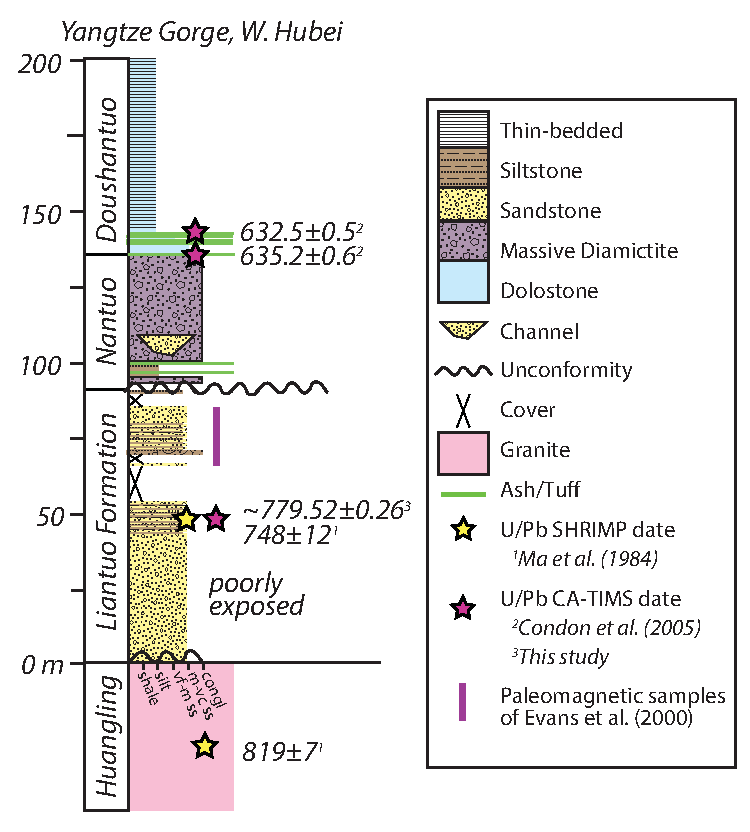
\includegraphics[width=0.8\textwidth]{figures/Xiajiang/FDM14-1-strat.pdf}
    \caption[Tonian-Cryogenian stratigraphy of the Yangtze Gorge.]{Tonian-Cryogenian stratigraphy of the Yangtze Gorge, from where the paleomagnetic and geochronologic data for the Liantuo Formation are developed.}
    \label{fig:FDM14-1-strat}
\end{figure}

\begin{sidewaystable*}[h!]
\tiny
\vspace*{1 cm}
\caption{U-Pb data for analyzed zircons from H2-470.}
\vspace{1 cm}
\setlength\tabcolsep{3.5pt}
\begin{tabular}{cccccccccccccccccccc}
& \multicolumn{8}{l}{Dates (Ma)} & \multicolumn{4}{l}{Composition} & \multicolumn{7}{l}{Isotopic Ratios} \\
\cline{2-20}\\
& $^a$ & & $^b$ & & $^{a,b}$ & & & $^c$ & $^d$ & $^e$ & $^f$ & $^{g}$ & $^h$ & $^{a,i}$ & & $^{b,i}$ & & $^{a,b,i}$ & \\	
& \underline{$^{206}$Pb} & $\pm$ & \underline{$^{207}$Pb} & $\pm$ & \underline{$^{207}$Pb} & $\pm$ & corr. & & \underline{Th} & Pb\** & Pb$_c$ & \underline{Pb\**} & \underline{$^{206}$Pb} & \underline{$^{206}$Pb} & $\pm$ & \underline{$^{207}$Pb} & $\pm$ & \underline{$^{207}$Pb} & $\pm$ \\		
fraction & $^{238}$U & (2$\sigma$) & $^{235}$U & (2$\sigma$) & $^{206}$Pb & (2$\sigma$) & coef. & \% disc. & U & (pg) & (pg) & Pb$_c$ & $^{204}$Pb & $^{238}$Pb & (2$\sigma\%$) & $^{235}$U & (2$\sigma\%$) & $^{206}$Pb & (2$\sigma\%$) \\
\hline \\
z9  & 809.55 & 0.53 & 811.00 & 1.10 & 814.95 & 3.88 & 0.33 & 0.69  & 0.90 & 15.6  & 0.25 & 62.2   & 3392  & 0.133808 & 0.070220 & 1.222669 & 0.196189 & 0.066301 & 0.182537 \\
z11 & 814.18 & 0.34 & 814.14 & 0.70 & 814.03 & 2.46 & 0.34 & 0.01  & 0.74 & 24.5  & 0.17 & 141.8  & 7993  & 0.134622 & 0.044107 & 1.229565 & 0.125086 & 0.066272 & 0.113043 \\
\rowcolor{Yellow}
z14 & 815.23 & 0.52 & 815.70 & 0.71 & 816.99 & 2.14 & 0.59 & 0.25  & 0.77 & 151.5 & 0.32 & 479.9  & 26838 & 0.134807 & 0.067705 & 1.232995 & 0.126378 & 0.066366 & 0.096844 \\
\rowcolor{Yellow}
z2  & 815.35 & 0.54 & 815.71 & 0.80 & 816.70 & 1.69 & 0.93 & 0.20  & 0.58 & 181.3 & 0.18 & 1013.2 & 59304 & 0.134828 & 0.070797 & 1.233019 & 0.143199 & 0.066356 & 0.074214 \\
\rowcolor{Yellow}
z3  & 815.62 & 0.72 & 816.98 & 2.39 & 820.70 & 8.28 & 0.41 & 0.65  & 0.62 & 95.6  & 5.15 & 18.6   & 1093  & 0.134876 & 0.093966 & 1.235816 & 0.424989 & 0.066484 & 0.394981 \\
\rowcolor{Yellow}
z7  & 815.73 & 0.99 & 815.63 & 0.88 & 815.35 & 1.90 & 0.82 & -0.02 & 0.88 & 38.7  & 0.30 & 128.9  & 7036  & 0.134895 & 0.128998 & 1.232832 & 0.157563 & 0.066314 & 0.084703 \\
\rowcolor{Yellow}
z8  & 815.85 & 0.27 & 815.87 & 0.40 & 815.92 & 1.25 & 0.53 & 0.04  & 0.72 & 35.1  & 0.15 & 226.9  & 12842 & 0.134917 & 0.035031 & 1.233366 & 0.070632 & 0.066332 & 0.050324 \\
\rowcolor{Yellow}
z12 & 815.93 & 0.36 & 815.43 & 0.56 & 814.06 & 1.78 & 0.54 & -0.20 & 0.78 & 23.6  & 0.16 & 148.4  & 8295  & 0.134931 & 0.047158 & 1.232398 & 0.100758 & 0.066273 & 0.078418 \\
z1  & 816.69 & 0.53 & 816.90 & 0.84 & 817.48 & 1.95 & 0.90 & 0.13  & 0.76 & 132.2 & 0.74 & 179.4  & 10069 & 0.135064 & 0.069554 & 1.235639 & 0.150465 & 0.066381 & 0.087256 \\
z4  & 816.73 & 0.61 & 816.60 & 0.88 & 816.24 & 2.11 & 0.83 & -0.03 & 0.73 & 32.6  & 0.12 & 272.7  & 15417 & 0.135072 & 0.079228 & 1.234975 & 0.156380 & 0.066342 & 0.095355 \\
z6  & 817.69 & 0.34 & 817.70 & 0.42 & 817.73 & 1.19 & 0.65 & 0.04  & 0.86 & 60.2  & 0.26 & 232.1  & 12723 & 0.135239 & 0.044110 & 1.237385 & 0.074873 & 0.066389 & 0.046714 \\
z5  & 818.04 & 0.54 & 818.01 & 0.80 & 817.92 & 1.78 & 0.90 & 0.02  & 0.72 & 57.6  & 0.14 & 408.6  & 23141 & 0.135301 & 0.070555 & 1.238068 & 0.143195 & 0.066395 & 0.078665 \\
z10 & 818.13 & 0.30 & 817.69 & 0.44 & 816.47 & 1.32 & 0.62 & -0.17 & 0.76 & 50.0  & 0.16 & 311.7  & 17475 & 0.135318 & 0.038917 & 1.237363 & 0.079176 & 0.066349 & 0.053969 \\
z16 & 826.68 & 0.32 & 824.61 & 0.43 & 819.04 & 1.27 & 0.61 & -0.90 & 0.74 & 93.5  & 0.30 & 311.7  & 17581 & 0.136824 & 0.040989 & 1.252669 & 0.076810 & 0.066431 & 0.051484 \\
z13 & 830.20 & 0.53 & 825.34 & 0.85 & 812.27 & 2.03 & 0.87 & -2.17 & 0.75 & 62.5  & 0.38 & 164.3  & 9250  & 0.137445 & 0.068375 & 1.254296 & 0.149999 & 0.066216 & 0.091207 \\
z15 & 844.63 & 0.31 & 837.47 & 0.90 & 818.55 & 3.17 & 0.28 & -3.16 & 1.03 & 41.3  & 0.76 & 54.4   & 2879  & 0.139994 & 0.038917 & 1.281393 & 0.158093 & 0.066415 & 0.148349 \\
\end{tabular}

\flushleft \emph{Notes:} \\
Colored rows indicate fractions included in the calculation of the reported sample age. \\
Isotopic dates calculated using $\lambda$238 = 1.55125$\times$10$^{-10}$ and $\lambda$235 = 9.8485$\times$10$^{-10}$ \citep{Jaffey1971a}. \\
 $^{a}$  Corrected for initial Th/U disequilibrium using radiogenic $^{208}$Pb and Th/U[magma] = 2.8. \\
 $^{b}$ Corrected for initial Pa/U disequilibrium using initial fraction activity ratio [$^{231}$Pa]/[$^{235}$U] = 1.10000. \\
 $^{c}$ \% discordance = 100 - (100 $\times$ ($^{206}$Pb/$^{238}$U date) / ($^{207}$Pb/$^{206}$Pb date)) \\
 $^{d}$ Th contents calculated from radiogenic $^{208}$Pb and $^{230}$Th-corrected $^{206}$Pb/$^{238}$U date of the sample, assuming concordance between U-Pb Th-Pb systems. \\
 $^{e}$ Total mass of radiogenic Pb. \\
 $^{f}$ Total mass of common Pb. \\
 $^{g}$ Ratio of radiogenic Pb (including $^{208}$Pb) to common Pb. \\
 $^{h}$ Measured ratio corrected for fractionation and spike contribution only. \\
 $^{i}$ Measured ratios corrected for fractionation, tracer and blank.
\end{sidewaystable*}

\begin{sidewaystable*}[h!]
\tiny
\vspace*{1 cm}
\caption{U-Pb data for analyzed zircons from L1-27.}
\vspace{1 cm}
\setlength\tabcolsep{3.5pt}
\begin{tabular}{cccccccccccccccccccc}
& \multicolumn{8}{l}{Dates (Ma)} & \multicolumn{4}{l}{Composition} & \multicolumn{7}{l}{Isotopic Ratios} \\
\cline{2-20}\\
& $^a$ & & $^b$ & & $^{a,b}$ & & & $^c$ & $^d$ & $^e$ & $^f$ & $^{g}$ & $^h$ & $^{a,i}$ & & $^{b,i}$ & & $^{a,b,i}$ & \\	
& \underline{$^{206}$Pb} & $\pm$ & \underline{$^{207}$Pb} & $\pm$ & \underline{$^{207}$Pb} & $\pm$ & corr. & & \underline{Th} & Pb\** & Pb$_c$ & \underline{Pb\**} & \underline{$^{206}$Pb} & \underline{$^{206}$Pb} & $\pm$ & \underline{$^{207}$Pb} & $\pm$ & \underline{$^{207}$Pb} & $\pm$ \\		
fraction & $^{238}$U & (2$\sigma$) & $^{235}$U & (2$\sigma$) & $^{206}$Pb & (2$\sigma$) & coef. & \% disc. & U & (pg) & (pg) & Pb$_c$ & $^{204}$Pb & $^{238}$Pb & (2$\sigma\%$) & $^{235}$U & (2$\sigma\%$) & $^{206}$Pb & (2$\sigma\%$) \\
\hline \\
z5  & 804.84 & 0.56 & 806.95 & 1.16 & 812.78 & 3.42  & 0.72 & 1.01  & 0.73 & 50.5 & 0.82 & 61.7  & 3500 & 0.132980 & 0.073384 & 1.213839 & 0.207803 & 0.066232 & 0.160083 \\
z6  & 807.82 & 0.91 & 808.27 & 4.24 & 809.52 & 15.58 & 0.22 & 0.24  & 0.79 & 7.0  & 0.63 & 11.1  & 638  & 0.133504 & 0.119942 & 1.216721 & 0.761579 & 0.066129 & 0.744112 \\
\rowcolor{Yellow}
z9  & 813.90 & 0.39 & 813.80 & 0.88 & 813.52 & 3.20  & 0.22 & -0.02 & 0.85 & 27.2 & 0.32 & 85.4  & 4697 & 0.134572 & 0.050696 & 1.228808 & 0.156387 & 0.066256 & 0.149699 \\
\rowcolor{Yellow}
z8  & 814.06 & 0.48 & 813.32 & 1.08 & 811.29 & 3.66  & 0.43 & -0.31 & 0.98 & 16.3 & 0.31 & 52.0  & 2787 & 0.134600 & 0.062729 & 1.227755 & 0.192831 & 0.066185 & 0.172067 \\
\rowcolor{Yellow}
z2  & 814.11 & 0.53 & 814.33 & 0.83 & 814.92 & 1.97  & 0.88 & 0.13  & 0.62 & 55.9 & 0.33 & 169.6 & 9852 & 0.134610 & 0.068803 & 1.229970 & 0.148922 & 0.066300 & 0.088455 \\
\rowcolor{Yellow}
z12 & 814.55 & 0.67 & 814.81 & 0.99 & 815.50 & 3.29  & 0.46 & 0.14  & 1.10 & 18.0 & 0.26 & 68.8  & 3583 & 0.134688 & 0.087437 & 1.231029 & 0.177274 & 0.066318 & 0.153859 \\
\rowcolor{Yellow}
z11 & 814.57 & 0.44 & 814.14 & 0.70 & 812.95 & 2.47  & 0.35 & -0.17 & 0.87 & 19.5 & 0.23 & 86.0  & 4714 & 0.134691 & 0.058009 & 1.229554 & 0.125152 & 0.066238 & 0.113683 \\
z4  & 815.24 & 0.59 & 814.91 & 1.15 & 814.02 & 3.28  & 0.75 & -0.12 & 0.84 & 18.9 & 0.27 & 71.1  & 3926 & 0.134808 & 0.076864 & 1.231253 & 0.205803 & 0.066271 & 0.153331 \\
z7  & 815.75 & 0.53 & 814.78 & 1.43 & 812.13 & 5.12  & 0.27 & -0.41 & 0.88 & 9.1  & 0.27 & 33.0  & 1818 & 0.134898 & 0.069355 & 1.230966 & 0.254447 & 0.066212 & 0.242857 \\
\end{tabular}

\flushleft \emph{Notes:} \\
Colored rows indicate fractions included in the calculation of the reported sample age. \\
Isotopic dates calculated using $\lambda$238 = 1.55125$\times$10$^{-10}$ and $\lambda$235 = 9.8485$\times$10$^{-10}$ \citep{Jaffey1971a}. \\
 $^{a}$  Corrected for initial Th/U disequilibrium using radiogenic $^{208}$Pb and Th/U[magma] = 2.8. \\
 $^{b}$ Corrected for initial Pa/U disequilibrium using initial fraction activity ratio [$^{231}$Pa]/[$^{235}$U] = 1.10000. \\
 $^{c}$ \% discordance = 100 - (100 $\times$ ($^{206}$Pb/$^{238}$U date) / ($^{207}$Pb/$^{206}$Pb date)) \\
 $^{d}$ Th contents calculated from radiogenic $^{208}$Pb and $^{230}$Th-corrected $^{206}$Pb/$^{238}$U date of the sample, assuming concordance between U-Pb Th-Pb systems. \\
 $^{e}$ Total mass of radiogenic Pb. \\
 $^{f}$ Total mass of common Pb. \\
 $^{g}$ Ratio of radiogenic Pb (including $^{208}$Pb) to common Pb. \\
 $^{h}$ Measured ratio corrected for fractionation and spike contribution only. \\
 $^{i}$ Measured ratios corrected for fractionation, tracer and blank.
\end{sidewaystable*}

\begin{sidewaystable*}[h!]
\tiny
\vspace*{1 cm}
\caption{U-Pb data for analyzed zircons from L4-2.}
\vspace{1 cm}
\setlength\tabcolsep{3.5pt}
\begin{tabular}{cccccccccccccccccccc}
& \multicolumn{8}{l}{Dates (Ma)} & \multicolumn{4}{l}{Composition} & \multicolumn{7}{l}{Isotopic Ratios} \\
\cline{2-20}\\
& $^a$ & & $^b$ & & $^{a,b}$ & & & $^c$ & $^d$ & $^e$ & $^f$ & $^{g}$ & $^h$ & $^{a,i}$ & & $^{b,i}$ & & $^{a,b,i}$ & \\	
& \underline{$^{206}$Pb} & $\pm$ & \underline{$^{207}$Pb} & $\pm$ & \underline{$^{207}$Pb} & $\pm$ & corr. & & \underline{Th} & Pb\** & Pb$_c$ & \underline{Pb\**} & \underline{$^{206}$Pb} & \underline{$^{206}$Pb} & $\pm$ & \underline{$^{207}$Pb} & $\pm$ & \underline{$^{207}$Pb} & $\pm$ \\		
fraction & $^{238}$U & (2$\sigma$) & $^{235}$U & (2$\sigma$) & $^{206}$Pb & (2$\sigma$) & coef. & \% disc. & U & (pg) & (pg) & Pb$_c$ & $^{204}$Pb & $^{238}$Pb & (2$\sigma\%$) & $^{235}$U & (2$\sigma\%$) & $^{206}$Pb & (2$\sigma\%$) \\
\hline \\
\rowcolor{Yellow}
z5 & 812.67 & 0.73 & 812.99 & 0.96 & 813.86 & 2.20 & 0.84 & 0.18  & 0.64 & 28.3 & 0.17 & 170.0 & 9812 & 0.134357 & 0.096183 & 1.227035 & 0.171839 & 0.066266 & 0.100134 \\
\rowcolor{Yellow}
z3 & 812.88 & 0.57 & 812.67 & 0.88 & 812.09 & 2.13 & 0.85 & -0.07 & 0.76 & 96.5 & 0.70 & 137.1 & 7703 & 0.134393 & 0.074304 & 1.226330 & 0.157528 & 0.066210 & 0.096556 \\
\rowcolor{Yellow}
z1 & 813.47 & 0.57 & 813.40 & 0.89 & 813.19 & 2.27 & 0.81 & 0.00  & 0.79 & 72.4 & 0.46 & 157.4 & 8784 & 0.134497 & 0.074341 & 1.227932 & 0.159174 & 0.066245 & 0.103450 \\
z4 & 817.05 & 1.02 & 817.05 & 2.02 & 817.07 & 5.95 & 0.70 & 0.03  & 0.78 & 10.7 & 0.25 & 43.5  & 2442 & 0.135127 & 0.132953 & 1.235972 & 0.360619 & 0.066368 & 0.282745 \\
\end{tabular}

\flushleft \emph{Notes:} \\
Colored rows indicate fractions included in the calculation of the reported sample age. \\
Isotopic dates calculated using $\lambda$238 = 1.55125$\times$10$^{-10}$ and $\lambda$235 = 9.8485$\times$10$^{-10}$ \citep{Jaffey1971a}. \\
 $^{a}$  Corrected for initial Th/U disequilibrium using radiogenic $^{208}$Pb and Th/U[magma] = 2.8. \\
 $^{b}$ Corrected for initial Pa/U disequilibrium using initial fraction activity ratio [$^{231}$Pa]/[$^{235}$U] = 1.10000. \\
 $^{c}$ \% discordance = 100 - (100 $\times$ ($^{206}$Pb/$^{238}$U date) / ($^{207}$Pb/$^{206}$Pb date)) \\
 $^{d}$ Th contents calculated from radiogenic $^{208}$Pb and $^{230}$Th-corrected $^{206}$Pb/$^{238}$U date of the sample, assuming concordance between U-Pb Th-Pb systems. \\
 $^{e}$ Total mass of radiogenic Pb. \\
 $^{f}$ Total mass of common Pb. \\
 $^{g}$ Ratio of radiogenic Pb (including $^{208}$Pb) to common Pb. \\
 $^{h}$ Measured ratio corrected for fractionation and spike contribution only. \\
 $^{i}$ Measured ratios corrected for fractionation, tracer and blank.
\end{sidewaystable*}

\begin{sidewaystable*}[h!]
\tiny
\vspace*{1 cm}
\caption{U-Pb data for analyzed zircons from QR-74.}
\vspace{1 cm}
\setlength\tabcolsep{3.5pt}
\begin{tabular}{cccccccccccccccccccc}
& \multicolumn{8}{l}{Dates (Ma)} & \multicolumn{4}{l}{Composition} & \multicolumn{7}{l}{Isotopic Ratios} \\
\cline{2-20}\\
& $^a$ & & $^b$ & & $^{a,b}$ & & & $^c$ & $^d$ & $^e$ & $^f$ & $^{g}$ & $^h$ & $^{a,i}$ & & $^{b,i}$ & & $^{a,b,i}$ & \\	
& \underline{$^{206}$Pb} & $\pm$ & \underline{$^{207}$Pb} & $\pm$ & \underline{$^{207}$Pb} & $\pm$ & corr. & & \underline{Th} & Pb\** & Pb$_c$ & \underline{Pb\**} & \underline{$^{206}$Pb} & \underline{$^{206}$Pb} & $\pm$ & \underline{$^{207}$Pb} & $\pm$ & \underline{$^{207}$Pb} & $\pm$ \\		
fraction & $^{238}$U & (2$\sigma$) & $^{235}$U & (2$\sigma$) & $^{206}$Pb & (2$\sigma$) & coef. & \% disc. & U & (pg) & (pg) & Pb$_c$ & $^{204}$Pb & $^{238}$Pb & (2$\sigma\%$) & $^{235}$U & (2$\sigma\%$) & $^{206}$Pb & (2$\sigma\%$) \\
\hline \\
z3  & 804.83 & 1.24 & 805.14 & 3.41  & 806.01 & 11.84 & 0.42 & 0.17  & 1.23 & 22.8 & 1.33 & 17.1  & 879  & 0.132978 & 0.163397 & 1.209897 & 0.614028 & 0.066018 & 0.564721 \\
\rowcolor{Yellow}
z16 & 810.71 & 1.64 & 808.35 & 4.05  & 801.85 & 13.64 & 0.48 & -1.08 & 1.51 & 4.5  & 0.27 & 16.9  & 821  & 0.134012 & 0.215638 & 1.216885 & 0.726288 & 0.065887 & 0.650260 \\
\rowcolor{Yellow}
z11 & 810.75 & 1.28 & 812.97 & 4.90  & 819.06 & 17.07 & 0.44 & 1.02  & 2.16 & 4.4  & 0.29 & 15.3  & 661  & 0.134018 & 0.168352 & 1.226995 & 0.876654 & 0.066431 & 0.816287 \\
\rowcolor{Yellow}
z2  & 812.05 & 0.90 & 809.95 & 2.91  & 804.18 & 9.90  & 0.51 & -0.95 & 0.78 & 6.1  & 0.23 & 26.3  & 1483 & 0.134247 & 0.117602 & 1.220376 & 0.521619 & 0.065960 & 0.471892 \\
z8  & 820.43 & 0.67 & 821.41 & 1.00  & 824.08 & 2.43  & 0.82 & 0.48  & 0.53 & 51.0 & 0.34 & 151.9 & 9025 & 0.135722 & 0.086584 & 1.245585 & 0.176779 & 0.066591 & 0.111640 \\
z12 & 851.34 & 3.08 & 860.05 & 15.02 & 882.58 & 52.25 & 0.23 & 3.57  & 0.82 & 4.8  & 1.62 & 3.0   & 182  & 0.141182 & 0.386791 & 1.332696 & 2.588865 & 0.068493 & 2.526201 \\
\end{tabular}

\flushleft \emph{Notes:} \\
Colored rows indicate fractions included in the calculation of the reported sample age. \\
Isotopic dates calculated using $\lambda$238 = 1.55125$\times$10$^{-10}$ and $\lambda$235 = 9.8485$\times$10$^{-10}$ \citep{Jaffey1971a}. \\
 $^{a}$  Corrected for initial Th/U disequilibrium using radiogenic $^{208}$Pb and Th/U[magma] = 2.8. \\
 $^{b}$ Corrected for initial Pa/U disequilibrium using initial fraction activity ratio [$^{231}$Pa]/[$^{235}$U] = 1.10000. \\
 $^{c}$ \% discordance = 100 - (100 $\times$ ($^{206}$Pb/$^{238}$U date) / ($^{207}$Pb/$^{206}$Pb date)) \\
 $^{d}$ Th contents calculated from radiogenic $^{208}$Pb and $^{230}$Th-corrected $^{206}$Pb/$^{238}$U date of the sample, assuming concordance between U-Pb Th-Pb systems. \\
 $^{e}$ Total mass of radiogenic Pb. \\
 $^{f}$ Total mass of common Pb. \\
 $^{g}$ Ratio of radiogenic Pb (including $^{208}$Pb) to common Pb. \\
 $^{h}$ Measured ratio corrected for fractionation and spike contribution only. \\
 $^{i}$ Measured ratios corrected for fractionation, tracer and blank.
\end{sidewaystable*}

\begin{sidewaystable*}[h!]
\tiny
\vspace*{1 cm}
\caption{U-Pb data for analyzed zircons from H3-60.}
\vspace{1 cm}
\setlength\tabcolsep{3.5pt}
\begin{tabular}{cccccccccccccccccccc}
& \multicolumn{8}{l}{Dates (Ma)} & \multicolumn{4}{l}{Composition} & \multicolumn{7}{l}{Isotopic Ratios} \\
\cline{2-20}\\
& $^a$ & & $^b$ & & $^{a,b}$ & & & $^c$ & $^d$ & $^e$ & $^f$ & $^{g}$ & $^h$ & $^{a,i}$ & & $^{b,i}$ & & $^{a,b,i}$ & \\	
& \underline{$^{206}$Pb} & $\pm$ & \underline{$^{207}$Pb} & $\pm$ & \underline{$^{207}$Pb} & $\pm$ & corr. & & \underline{Th} & Pb\** & Pb$_c$ & \underline{Pb\**} & \underline{$^{206}$Pb} & \underline{$^{206}$Pb} & $\pm$ & \underline{$^{207}$Pb} & $\pm$ & \underline{$^{207}$Pb} & $\pm$ \\		
fraction & $^{238}$U & (2$\sigma$) & $^{235}$U & (2$\sigma$) & $^{206}$Pb & (2$\sigma$) & coef. & \% disc. & U & (pg) & (pg) & Pb$_c$ & $^{204}$Pb & $^{238}$Pb & (2$\sigma\%$) & $^{235}$U & (2$\sigma\%$) & $^{206}$Pb & (2$\sigma\%$) \\
\hline \\
\rowcolor{Yellow}
z89 & 808.42  & 1.31 & 811.45  & 5.14  & 819.76  & 18.09  & 0.40 & 1.41  & 0.90 & 5.4  & 0.52 & 10.3 & 576  & 0.133609 & 0.172358 & 1.223662 & 0.920442 & 0.066454 & 0.865681 \\
\rowcolor{Yellow}
z5  & 808.51  & 1.29 & 804.95  & 5.58  & 795.10  & 19.50  & 0.51 & -1.66 & 1.19 & 6.8  & 0.46 & 14.6 & 763  & 0.133625 & 0.169577 & 1.209472 & 1.004012 & 0.065675 & 0.929277 \\
\rowcolor{Yellow}
z6  & 809.60  & 0.85 & 811.12  & 2.63  & 815.31  & 8.74   & 0.57 & 0.72  & 1.64 & 6.3  & 0.22 & 28.5 & 1338 & 0.133816 & 0.111624 & 1.222945 & 0.471028 & 0.066312 & 0.416759 \\
\rowcolor{Yellow}
z4  & 810.15  & 1.17 & 806.92  & 4.41  & 798.04  & 15.31  & 0.48 & -1.49 & 1.06 & 5.6  & 0.42 & 13.5 & 723  & 0.133912 & 0.154026 & 1.213773 & 0.791331 & 0.065767 & 0.729865 \\
\rowcolor{Yellow}
z3  & 810.55  & 1.28 & 805.72  & 6.14  & 792.41  & 21.33  & 0.57 & -2.25 & 0.70 & 5.2  & 0.48 & 10.9 & 639  & 0.133983 & 0.168169 & 1.211159 & 1.103179 & 0.065591 & 1.016252 \\
\rowcolor{Yellow}
z9  & 810.99  & 6.08 & 822.57  & 34.27 & 854.01  & 115.84 & 0.67 & 5.06  & 0.97 & 3.7  & 0.72 & 5.2  & 293  & 0.134062 & 0.797956 & 1.248158 & 6.078624 & 0.067555 & 5.576013 \\
z24 & 813.41  & 0.75 & 815.79  & 1.91  & 822.30  & 6.02   & 0.63 & 1.12  & 0.18 & 7.8  & 0.24 & 33.0 & 2158 & 0.134487 & 0.098631 & 1.233197 & 0.339772 & 0.066535 & 0.286461 \\
z30 & 832.33  & 3.35 & 836.95  & 5.23  & 849.22  & 15.68  & 0.58 & 2.02  & 0.53 & 5.2  & 0.33 & 15.8 & 956  & 0.137821 & 0.428971 & 1.280210 & 0.916686 & 0.067400 & 0.753347 \\
z2  & 1686.09 & 2.05 & 1687.11 & 3.57  & 1688.38 & 7.24   & 0.45 & 0.14  & 0.82 & 12.2 & 0.86 & 14.2 & 789  & 0.298948 & 0.138089 & 4.267470 & 0.433978 & 0.103578 & 0.391116 \\
\end{tabular}

\flushleft \emph{Notes:} \\
Colored rows indicate fractions included in the calculation of the reported sample age. \\
Isotopic dates calculated using $\lambda$238 = 1.55125$\times$10$^{-10}$ and $\lambda$235 = 9.8485$\times$10$^{-10}$ \citep{Jaffey1971a}. \\
 $^{a}$  Corrected for initial Th/U disequilibrium using radiogenic $^{208}$Pb and Th/U[magma] = 2.8. \\
 $^{b}$ Corrected for initial Pa/U disequilibrium using initial fraction activity ratio [$^{231}$Pa]/[$^{235}$U] = 1.10000. \\
 $^{c}$ \% discordance = 100 - (100 $\times$ ($^{206}$Pb/$^{238}$U date) / ($^{207}$Pb/$^{206}$Pb date)) \\
 $^{d}$ Th contents calculated from radiogenic $^{208}$Pb and $^{230}$Th-corrected $^{206}$Pb/$^{238}$U date of the sample, assuming concordance between U-Pb Th-Pb systems. \\
 $^{e}$ Total mass of radiogenic Pb. \\
 $^{f}$ Total mass of common Pb. \\
 $^{g}$ Ratio of radiogenic Pb (including $^{208}$Pb) to common Pb. \\
 $^{h}$ Measured ratio corrected for fractionation and spike contribution only. \\
 $^{i}$ Measured ratios corrected for fractionation, tracer and blank.
\end{sidewaystable*}

\begin{sidewaystable*}[h!]
\tiny
\vspace*{1 cm}
\caption{U-Pb data for analyzed zircons from H3-8.}
\vspace{1 cm}
\setlength\tabcolsep{3.5pt}
\begin{tabular}{cccccccccccccccccccc}
& \multicolumn{8}{l}{Dates (Ma)} & \multicolumn{4}{l}{Composition} & \multicolumn{7}{l}{Isotopic Ratios} \\
\cline{2-20}\\
& $^a$ & & $^b$ & & $^{a,b}$ & & & $^c$ & $^d$ & $^e$ & $^f$ & $^{g}$ & $^h$ & $^{a,i}$ & & $^{b,i}$ & & $^{a,b,i}$ & \\	
& \underline{$^{206}$Pb} & $\pm$ & \underline{$^{207}$Pb} & $\pm$ & \underline{$^{207}$Pb} & $\pm$ & corr. & & \underline{Th} & Pb\** & Pb$_c$ & \underline{Pb\**} & \underline{$^{206}$Pb} & \underline{$^{206}$Pb} & $\pm$ & \underline{$^{207}$Pb} & $\pm$ & \underline{$^{207}$Pb} & $\pm$ \\		
fraction & $^{238}$U & (2$\sigma$) & $^{235}$U & (2$\sigma$) & $^{206}$Pb & (2$\sigma$) & coef. & \% disc. & U & (pg) & (pg) & Pb$_c$ & $^{204}$Pb & $^{238}$Pb & (2$\sigma\%$) & $^{235}$U & (2$\sigma\%$) & $^{206}$Pb & (2$\sigma\%$) \\
\hline \\
\rowcolor{Yellow}
z18 & 804.34 & 0.57 & 803.51 & 1.16 & 801.23 & 3.36  & 0.75 & -0.36 & 1.23 & 15.5 & 0.17 & 91.5 & 4632 & 0.132891 & 0.075104 & 1.206350 & 0.208574 & 0.065868 & 0.156792 \\
\rowcolor{Yellow}
z10 & 804.70 & 0.63 & 804.30 & 1.30 & 803.21 & 3.77  & 0.75 & -0.16 & 0.92 & 13.6 & 0.20 & 68.5 & 3713 & 0.132954 & 0.083190 & 1.208067 & 0.233224 & 0.065930 & 0.176835 \\
\rowcolor{Yellow}
z22 & 804.92 & 1.05 & 802.18 & 3.41 & 794.60 & 12.04 & 0.39 & -1.28 & 1.48 & 5.8  & 0.32 & 18.4 & 896  & 0.132993 & 0.138384 & 1.203463 & 0.614233 & 0.065660 & 0.573000 \\
z23 & 809.85 & 1.38 & 808.78 & 6.36 & 805.83 & 22.85 & 0.35 & -0.48 & 1.86 & 6.8  & 0.71 & 9.6  & 443  & 0.133861 & 0.181847 & 1.217825 & 1.141112 & 0.066012 & 1.090857 \\
\end{tabular}

\flushleft \emph{Notes:} \\
Colored rows indicate fractions included in the calculation of the reported sample age. \\
Isotopic dates calculated using $\lambda$238 = 1.55125$\times$10$^{-10}$ and $\lambda$235 = 9.8485$\times$10$^{-10}$ \citep{Jaffey1971a}. \\
 $^{a}$  Corrected for initial Th/U disequilibrium using radiogenic $^{208}$Pb and Th/U[magma] = 2.8. \\
 $^{b}$ Corrected for initial Pa/U disequilibrium using initial fraction activity ratio [$^{231}$Pa]/[$^{235}$U] = 1.10000. \\
 $^{c}$ \% discordance = 100 - (100 $\times$ ($^{206}$Pb/$^{238}$U date) / ($^{207}$Pb/$^{206}$Pb date)) \\
 $^{d}$ Th contents calculated from radiogenic $^{208}$Pb and $^{230}$Th-corrected $^{206}$Pb/$^{238}$U date of the sample, assuming concordance between U-Pb Th-Pb systems. \\
 $^{e}$ Total mass of radiogenic Pb. \\
 $^{f}$ Total mass of common Pb. \\
 $^{g}$ Ratio of radiogenic Pb (including $^{208}$Pb) to common Pb. \\
 $^{h}$ Measured ratio corrected for fractionation and spike contribution only. \\
 $^{i}$ Measured ratios corrected for fractionation, tracer and blank.
\end{sidewaystable*}

\begin{sidewaystable*}[h!]
\tiny
\vspace*{1 cm}
\caption{U-Pb data for analyzed zircons from ZJ-B.}
\vspace{1 cm}
\setlength\tabcolsep{3.5pt}
\begin{tabular}{cccccccccccccccccccc}
& \multicolumn{8}{l}{Dates (Ma)} & \multicolumn{4}{l}{Composition} & \multicolumn{7}{l}{Isotopic Ratios} \\
\cline{2-20}\\
& $^a$ & & $^b$ & & $^{a,b}$ & & & $^c$ & $^d$ & $^e$ & $^f$ & $^{g}$ & $^h$ & $^{a,i}$ & & $^{b,i}$ & & $^{a,b,i}$ & \\	
& \underline{$^{206}$Pb} & $\pm$ & \underline{$^{207}$Pb} & $\pm$ & \underline{$^{207}$Pb} & $\pm$ & corr. & & \underline{Th} & Pb\** & Pb$_c$ & \underline{Pb\**} & \underline{$^{206}$Pb} & \underline{$^{206}$Pb} & $\pm$ & \underline{$^{207}$Pb} & $\pm$ & \underline{$^{207}$Pb} & $\pm$ \\		
fraction & $^{238}$U & (2$\sigma$) & $^{235}$U & (2$\sigma$) & $^{206}$Pb & (2$\sigma$) & coef. & \% disc. & U & (pg) & (pg) & Pb$_c$ & $^{204}$Pb & $^{238}$Pb & (2$\sigma\%$) & $^{235}$U & (2$\sigma\%$) & $^{206}$Pb & (2$\sigma\%$) \\
\hline \\
z4 & 804.12 & 0.71 & 807.83 & 1.73 & 818.10 & 5.30  & 0.70 & 1.74  & 0.63 & 23.9 & 0.45 & 52.6  & 3059 & 0.132852 & 0.093875 & 1.215759 & 0.310700 & 0.066401 & 0.251380 \\
\rowcolor{Yellow}
z1 & 804.38 & 0.74 & 805.03 & 1.95 & 806.82 & 6.32  & 0.61 & 0.33  & 0.91 & 23.9 & 0.80 & 29.7  & 1625 & 0.132898 & 0.098018 & 1.209641 & 0.350970 & 0.066044 & 0.300053 \\
\rowcolor{Yellow}
z2 & 804.67 & 0.94 & 804.49 & 3.20 & 804.00 & 10.43 & 0.69 & -0.05 & 0.64 & 17.7 & 0.91 & 19.4  & 1139 & 0.132949 & 0.123690 & 1.208474 & 0.575486 & 0.065955 & 0.496957 \\
\rowcolor{Yellow}
z5 & 805.02 & 0.73 & 805.55 & 1.17 & 807.04 & 2.84  & 0.86 & 0.28  & 0.73 & 21.8 & 0.19 & 112.8 & 6380 & 0.133011 & 0.096723 & 1.210789 & 0.209739 & 0.066051 & 0.131559 \\
\rowcolor{Yellow}
z6 & 805.23 & 0.80 & 805.83 & 1.66 & 807.48 & 5.05  & 0.67 & 0.32  & 0.46 & 7.1  & 0.19 & 37.0  & 2252 & 0.133048 & 0.105500 & 1.211388 & 0.298218 & 0.066064 & 0.239004 \\
\rowcolor{Yellow}
z3 & 805.24 & 0.85 & 805.36 & 1.88 & 805.70 & 5.85  & 0.65 & 0.09  & 0.61 & 8.1  & 0.23 & 34.9  & 2047 & 0.133050 & 0.112228 & 1.210372 & 0.338296 & 0.066008 & 0.277395 \\
\end{tabular}

\flushleft \emph{Notes:} \\
Colored rows indicate fractions included in the calculation of the reported sample age. \\
Isotopic dates calculated using $\lambda$238 = 1.55125$\times$10$^{-10}$ and $\lambda$235 = 9.8485$\times$10$^{-10}$ \citep{Jaffey1971a}. \\
 $^{a}$  Corrected for initial Th/U disequilibrium using radiogenic $^{208}$Pb and Th/U[magma] = 2.8. \\
 $^{b}$ Corrected for initial Pa/U disequilibrium using initial fraction activity ratio [$^{231}$Pa]/[$^{235}$U] = 1.10000. \\
 $^{c}$ \% discordance = 100 - (100 $\times$ ($^{206}$Pb/$^{238}$U date) / ($^{207}$Pb/$^{206}$Pb date)) \\
 $^{d}$ Th contents calculated from radiogenic $^{208}$Pb and $^{230}$Th-corrected $^{206}$Pb/$^{238}$U date of the sample, assuming concordance between U-Pb Th-Pb systems. \\
 $^{e}$ Total mass of radiogenic Pb. \\
 $^{f}$ Total mass of common Pb. \\
 $^{g}$ Ratio of radiogenic Pb (including $^{208}$Pb) to common Pb. \\
 $^{h}$ Measured ratio corrected for fractionation and spike contribution only. \\
 $^{i}$ Measured ratios corrected for fractionation, tracer and blank.
\end{sidewaystable*}

\begin{sidewaystable*}[h!]
\tiny
\vspace*{1 cm}
\caption{U-Pb data for analyzed zircons from FDM14-1.}
\vspace{1 cm}
\setlength\tabcolsep{3.5pt}
\begin{tabular}{cccccccccccccccccccc}
& \multicolumn{8}{l}{Dates (Ma)} & \multicolumn{4}{l}{Composition} & \multicolumn{7}{l}{Isotopic Ratios} \\
\cline{2-20}\\
& $^a$ & & $^b$ & & $^{a,b}$ & & & $^c$ & $^d$ & $^e$ & $^f$ & $^{g}$ & $^h$ & $^{a,i}$ & & $^{b,i}$ & & $^{a,b,i}$ & \\	
& \underline{$^{206}$Pb} & $\pm$ & \underline{$^{207}$Pb} & $\pm$ & \underline{$^{207}$Pb} & $\pm$ & corr. & & \underline{Th} & Pb\** & Pb$_c$ & \underline{Pb\**} & \underline{$^{206}$Pb} & \underline{$^{206}$Pb} & $\pm$ & \underline{$^{207}$Pb} & $\pm$ & \underline{$^{207}$Pb} & $\pm$ \\		
fraction & $^{238}$U & (2$\sigma$) & $^{235}$U & (2$\sigma$) & $^{206}$Pb & (2$\sigma$) & coef. & \% disc. & U & (pg) & (pg) & Pb$_c$ & $^{204}$Pb & $^{238}$Pb & (2$\sigma\%$) & $^{235}$U & (2$\sigma\%$) & $^{206}$Pb & (2$\sigma\%$) \\
\hline \\
z1  & 748.40 & 0.56 & 750.56 & 1.03 & 757.00 & 3.75  & 0.40 & 1.17  & 0.90 & 13.3 & 0.27 & 48.4  & 2643 & 0.123103 & 0.079758 & 1.094230 & 0.193393 & 0.064496 & 0.174627 \\
z17 & 774.57 & 0.64 & 775.72 & 1.78 & 779.03 & 6.08  & 0.55 & 0.60  & 1.34 & 10.2 & 0.28 & 36.9  & 1837 & 0.127673 & 0.087745 & 1.146782 & 0.327690 & 0.065174 & 0.287456 \\
z3  & 776.24 & 0.63 & 775.95 & 0.96 & 775.12 & 3.20  & 0.52 & -0.11 & 0.80 & 19.3 & 0.29 & 67.0  & 3736 & 0.127964 & 0.086814 & 1.147263 & 0.177841 & 0.065054 & 0.148394 \\
z4  & 776.90 & 0.38 & 777.25 & 0.57 & 778.28 & 1.85  & 0.53 & 0.20  & 1.50 & 35.7 & 0.29 & 122.7 & 5865 & 0.128079 & 0.051515 & 1.150022 & 0.104146 & 0.065151 & 0.081958 \\
\rowcolor{Yellow}
z8  & 778.89 & 0.79 & 778.89 & 1.37 & 778.91 & 4.19  & 0.65 & 0.03  & 1.47 & 21.9 & 0.32 & 69.6  & 3356 & 0.128427 & 0.107511 & 1.153495 & 0.251404 & 0.065171 & 0.196734 \\
\rowcolor{Yellow}
z15 & 778.95 & 1.10 & 780.15 & 1.90 & 783.60 & 5.77  & 0.66 & 0.62  & 1.35 & 12.5 & 0.23 & 55.0  & 2722 & 0.128438 & 0.149779 & 1.156169 & 0.348632 & 0.065316 & 0.272817 \\
\rowcolor{Yellow}
z9  & 779.07 & 0.75 & 779.49 & 1.24 & 780.71 & 3.68  & 0.68 & 0.24  & 1.31 & 17.3 & 0.25 & 70.0  & 3485 & 0.128459 & 0.102629 & 1.154767 & 0.227019 & 0.065227 & 0.171853 \\
\rowcolor{Yellow}
z7  & 779.40 & 0.94 & 779.09 & 2.41 & 778.20 & 8.46  & 0.45 & -0.12 & 0.94 & 15.3 & 0.71 & 21.7  & 1184 & 0.128518 & 0.128658 & 1.153915 & 0.443332 & 0.065149 & 0.401136 \\
\rowcolor{Yellow}
z12 & 779.59 & 0.75 & 780.56 & 1.87 & 783.35 & 6.22  & 0.58 & 0.49  & 2.10 & 11.8 & 0.27 & 43.8  & 1878 & 0.128550 & 0.102596 & 1.157039 & 0.343867 & 0.065309 & 0.294178 \\
\rowcolor{Yellow}
z13 & 779.62 & 0.69 & 779.22 & 0.99 & 778.08 & 2.55  & 0.80 & -0.17 & 0.96 & 29.3 & 0.21 & 138.1 & 7403 & 0.128556 & 0.094531 & 1.154197 & 0.182605 & 0.065145 & 0.116756 \\
\rowcolor{Yellow}
z5  & 779.67 & 0.50 & 779.65 & 1.36 & 779.59 & 5.02  & 0.30 & 0.02  & 1.08 & 8.9  & 0.24 & 37.2  & 1956 & 0.128565 & 0.068319 & 1.155104 & 0.250693 & 0.065192 & 0.236781 \\
\rowcolor{Yellow}
z16 & 780.83 & 0.92 & 780.36 & 2.68 & 779.02 & 9.09  & 0.58 & -0.21 & 1.36 & 6.7  & 0.17 & 39.6  & 1960 & 0.128767 & 0.125367 & 1.156612 & 0.492453 & 0.065174 & 0.431265 \\
z2  & 781.21 & 1.32 & 781.79 & 2.05 & 783.45 & 6.58  & 0.56 & 0.32  & 1.11 & 6.8  & 0.17 & 40.0  & 2089 & 0.128833 & 0.178839 & 1.159647 & 0.376544 & 0.065312 & 0.311606 \\
z11 & 781.44 & 1.10 & 783.35 & 5.17 & 788.79 & 19.22 & 0.28 & 0.95  & 1.47 & 12.3 & 1.25 & 9.9   & 492  & 0.128874 & 0.149953 & 1.162970 & 0.947064 & 0.065478 & 0.915141 \\
z14 & 795.30 & 0.68 & 794.22 & 1.31 & 791.16 & 3.99  & 0.66 & -0.50 & 1.50 & 29.2 & 0.36 & 81.2  & 3889 & 0.131305 & 0.091416 & 1.186240 & 0.237625 & 0.065552 & 0.187365 \\
z6  & 795.65 & 1.51 & 792.55 & 2.85 & 783.85 & 9.14  & 0.57 & -1.48 & 1.12 & 31.0 & 1.14 & 27.1  & 1420 & 0.131365 & 0.202001 & 1.182660 & 0.517519 & 0.065324 & 0.433779 \\
\end{tabular}

\flushleft \emph{Notes:} \\
Colored rows indicate fractions included in the calculation of the reported sample age. \\
Isotopic dates calculated using $\lambda$238 = 1.55125$\times$10$^{-10}$ and $\lambda$235 = 9.8485$\times$10$^{-10}$ \citep{Jaffey1971a}. \\
 $^{a}$  Corrected for initial Th/U disequilibrium using radiogenic $^{208}$Pb and Th/U[magma] = 2.8. \\
 $^{b}$ Corrected for initial Pa/U disequilibrium using initial fraction activity ratio [$^{231}$Pa]/[$^{235}$U] = 1.10000. \\
 $^{c}$ \% discordance = 100 - (100 $\times$ ($^{206}$Pb/$^{238}$U date) / ($^{207}$Pb/$^{206}$Pb date)) \\
 $^{d}$ Th contents calculated from radiogenic $^{208}$Pb and $^{230}$Th-corrected $^{206}$Pb/$^{238}$U date of the sample, assuming concordance between U-Pb Th-Pb systems. \\
 $^{e}$ Total mass of radiogenic Pb. \\
 $^{f}$ Total mass of common Pb. \\
 $^{g}$ Ratio of radiogenic Pb (including $^{208}$Pb) to common Pb. \\
 $^{h}$ Measured ratio corrected for fractionation and spike contribution only. \\
 $^{i}$ Measured ratios corrected for fractionation, tracer and blank.
\end{sidewaystable*}

\begin{table}[h!]
\caption[Euler rotation parameters used in the Bitter Springs Stage true polar wander model.]{Euler rotation parameters used in the Bitter Springs Stage true polar wander model (Fig. 11 in the main text).}
\vspace{0.25cm}
\resizebox{0.6\linewidth}{!}{
    \begin{tabular}{lccccl}
    \hline
    \textbf{plate} & \textbf{age} & \textbf{latitude} & \textbf{longitude} & \textbf{angle} & \textbf{relative plate} \\
    & \textbf{(Ma)} & \textbf{($^{\circ}$N)} & \textbf{($^{\circ}$E)} & \textbf{($^{\circ}$)} & \\
    &&&&& \\
    spin axis & 755 & -7.6 & -178.33 & -16.15 & mantle \\
    spin axis & 794 & -7.6 & -178.33 & -16.15 & mantle \\
    spin axis & 796 & -0.57 & 133.44 & -36.55 & mantle \\
    spin axis & 809 & -0.57 & 133.44 & -36.55 & mantle \\
    spin axis & 811 & 90.0 & 0.0 & 0.0 & mantle \\
    spin axis & 821 & 90.0 & 0.0 & 0.0 & mantle \\
    Laurentia & 755 & 43.4821 & 151.0109 & -167.5558 & spin axis \\
    Laurentia & 790 & 57.7447 & 147.6911 & -175.862 & spin axis \\
    Laurentia & 821 & 57.7447 & 147.6911 & -175.862 & spin axis \\
    Greenland & 755 & 67.5 & -118.5 & -13.8 & Laurentia \\
    Greenland & 821 & 67.5 & -118.5 & -13.8 & Laurentia \\
    Amazonia & 755 & 11.97 & -47.01 & -110.66 & Laurentia \\
    Amazonia & 821 & 11.97 & -47.01 & -110.66 & Laurentia \\
    Parana Panema & 755 & 0.67 & 103.22 & -30.82 & Amazonia \\
    Parana Panema & 821 & 0.67 & 103.22 & -30.82 & Amazonia \\
    Rio de la Plata & 755 & 0.67 & 103.22 & -30.82 & Amazonia \\
    Rio de la Plata & 821 & 0.67 & 103.22 & -30.82 & Amazonia \\
    Baltica & 755 & 75.8 & -95.8 & -59.2 & Laurentia \\
    Baltica & 821 & 75.8 & -95.8 & -59.2 & Laurentia \\
    Scotland & 755 & 78.64 & 161.9 & -32.0 & Laurentia \\
    Scotland & 821 & 78.64 & 161.9 & -32.0 & Laurentia \\
    Svalbard & 755 & -81.0 & 125.0 & 68.0 & Laurentia \\
    Svalbard & 821 & -81.0 & 125.0 & 68.0 & Laurentia \\
    Siberia & 755 & 77.0 & 98.0 & 137.0 & Laurentia \\
    Siberia & 821 & 77.0 & 98.0 & 137.0 & Laurentia \\
    India & 755 & 65.3333 & 103.3222 & -29.8536 & spin axis \\
    India & 790 & 24.9082 & 119.6524 & -45.5154 & spin axis \\
    India & 805 & 24.9082 & 119.6524 & -45.5154 & spin axis \\
    India & 821 & 21.5338 & 130.446 & -67.842 & spin axis \\
    North China & 755 & 52.9462 & 27.2366 & 61.9218 & Laurentia \\
    North China & 821 & 52.9462 & 27.2366 & 61.9218 & Laurentia \\
    South China & 755 & 6.7224 & 77.6921 & 67.9571 & India \\
    South China & 821 & 6.7224 & 77.6921 & 67.9571 & India \\
    Kalahari & 755 & 15.102 & -25.2783 & -157.5464 & Laurentia \\
    Kalahari & 821 & 15.102 & -25.2783 & -157.5464 & Laurentia \\
    South Australia & 755 & -30.2638 & -19.1192 & -131.7445 & Laurentia \\
    South Australia & 821 & -30.2638 & -19.1192 & -131.7445 & Laurentia \\
    North Australia & 755 & -20.0 & 135.0 & -40.0 & South Australia \\
    North Australia & 821 & -20.0 & 135.0 & -40.0 & South Australia \\
    East Antarctica & 755 & -3.91 & 37.9 & 30.86 & South Australia \\
    East Antarctica & 821 & -3.91 & 37.9 & 30.86 & South Australia \\
    Rayner & 755 & 1.8434 & -165.1696 & -91.8395 & India \\
    Rayner & 821 & 1.8434 & -165.1696 & -91.8395 & India \\
    \hline
    \end{tabular}}

\scriptsize
\flushleft \emph{Notes:} \\
(1) Model is defined between 821~Ma and 755~Ma.\\
\label{tab:Eulers}
\end{table}